\documentclass[10pt]{article}
\usepackage[a4paper,margin=18mm]{geometry}
\usepackage[T1]{fontenc}
\usepackage{amsmath,amssymb,booktabs,array,xcolor,graphicx}
\usepackage{tikz}
\usetikzlibrary{arrows.meta,positioning}
\usepackage{float}
\usepackage[round,authoryear]{natbib}
\usepackage[colorlinks=true,linkcolor=blue,citecolor=blue,urlcolor=blue]{hyperref}
\setlength{\parindent}{0pt}
\setlength{\parskip}{5pt}
\definecolor{replyblue}{RGB}{0,65,165}
\definecolor{graphblue}{HTML}{0072B2}
\definecolor{graphgreen}{HTML}{009E73}
\definecolor{graphorange}{HTML}{D55E00}
\definecolor{graphgray}{HTML}{A6B1BA}
\tikzset{wlvariable/.style={circle,draw=graphgreen,fill=graphgreen!7,
 line width=.7pt,minimum size=7mm,inner sep=1pt,text=black,font=\small},
 row/.style={rectangle,rounded corners=1.5pt,draw=graphblue,fill=graphblue!7,
 line width=.7pt,minimum width=9mm,minimum height=6mm,inner sep=1pt,text=black,font=\small},
 added/.style={row,draw=graphorange,fill=graphorange!7},
 connection/.style={draw=graphgray,line width=.7pt},
 note/.style={text=black,font=\small,align=left}}
\newcommand{\WL}{\mathrm{WLsubtree}}
\newcommand{\toygraph}[7]{%
 \node[wlvariable] (#1v1) at (2.25,1.6) {#2};
 \node[wlvariable] (#1v2) at (2.25,0) {#3};
 \node[row] (#1r1) at (.25,1.6) {#4};
 \node[row] (#1r2) at (.25,0) {#5};
 \draw[connection] (#1r1)--(#1v1) (#1r1)--(#1v2)
                   (#1r2)--(#1v1) (#1r2)--(#1v2);
 \ifnum#6=1
  \node[added] (#1r3) at (.25,-.85) {#7};
  \draw[graphorange,line width=1pt] (#1r3)--(#1v1);
 \fi}
\begin{document}
\textbf{\large Response to the Associate Editor: within-category heterogeneity}

\textit{Structural results verified on 6 October 2026.}

\textbf{Comment.} \textit{The second question concerns the heterogeneity of
problems even within each category. In my opinion, the reason that the
proposed method performed quite well may be attributed to the close
resemblance between the reference problem and the actual problem. However,
in reality, even when two problems belong to the same category, they can
still be drastically different. For example, there could be many additional
constraints, varying objectives, or other business requirements one may
consider in one type of problem. Would the current approach be robust
facing such conditions? How well can it perform? I didn't see clear evidence
from the current paper. I hope that the authors can also perform some tests
to analyze such scenarios.}

\begingroup\color{replyblue}
\textbf{Response.} We agree that a shared category does not establish a shared
formulation, and that the possibility of reference resemblance deserves a
direct examination. We therefore computed a Weisfeiler--Lehman (WL)
structural diagnostic for all 101 Large-Scale-OR benchmark formulations,
36 task variants, and the 15 LP files corresponding to the current
reference collection. To control for different ways of exporting variable
bounds, we analyze two consistently normalized representations and report
them separately: bounds retained in the \texttt{Bounds} section, and bounds
represented as explicit constraint rows. We also distinguish these
structural diagnostics from the complementary performance tests involving
task variants, leave-one-type-out (LOTO) evaluation, and forced routing.

\medskip
\textbf{Why a WL diagnostic is appropriate.}
The method combines two established components. Variable--constraint
bipartite graphs provide a natural way to represent MILP interactions
\citep{Gasse2019}. WL subtree kernels compare labeled graphs through
counts of progressively refined neighborhood patterns
\citep{Shervashidze2011}. Their combination allows us to compare explicit
formulation structure without relying on natural-language descriptions
or variable names.

Related MILP research learns graph-based instance similarities for
nearest-neighbor solver configuration \citep{Hosny2024}. That study
motivates comparing MILP instance representations, but uses a learned
metric related to solver costs. Here we choose an untrained WL feature
map so that every matched pattern and every calculation can be audited.
We use the literature to justify the representation and comparison
mechanism; it does not validate our scores as measures of business
semantics or solver performance.

The limitations are also grounded in MILP representation research.
\citet{Chen2023} show that their GNN class can fail to distinguish MILPs
with different feasibility properties. A recent arXiv manuscript by
\citet{Jahin2026}, whose record reports acceptance at TAG-DS 2026,
characterizes a class of MILP graph-transformer encoders as 1-WL bounded
under its stated input and architectural assumptions. These are
expressiveness results, not calibrations of a similarity threshold.
We accordingly use WL as a diagnostic of the selected labeled support
graph and retain these boundaries when interpreting the results.

\medskip
\textbf{Graph construction used in our implementation.}
We first apply the same bound-normalization rule to every reference,
benchmark instance, and variant. A linear row with exactly one nonzero
coefficient is converted to a bound: for example, $2x_j\leq6$ becomes
$x_j\leq3$, while a negative coefficient reverses the inequality.
Singleton equalities become coincident lower and upper bounds.
We intersect these restrictions with the native bounds, taking the
largest lower bound and the smallest upper bound. We then create two
representations:
\begin{enumerate}
\item \textbf{Bounds excluded from the graph.}
All effective bounds are stored in \texttt{Bounds}; their original
singleton rows are removed. Bounds still restrict the optimization
problem, but do not create graph nodes or edges. Finite bounds of integer
variables are represented by their ceiling/floor endpoints, preserving
the feasible integer lattice.
\item \textbf{Bounds included as constraint rows.}
Each effective finite lower and upper bound produces one explicit
inequality row. This includes default nonnegativity and binary $0/1$
bounds. Continuous and general integer variables are otherwise declared
free in \texttt{Bounds}; binary variables retain their intrinsic binary
domain. A fixed variable remains a variable node and has two coincident
bound rows. Duplicate or weaker singleton restrictions are not counted
again.
\end{enumerate}
Both representations retain variable domains, all remaining linear rows,
and all objectives. We do not perform general presolving, eliminate fixed
or isolated variables, or infer further bounds from multivariable rows.
Consequently, this normalization removes dependence on the storage
location and scaling of singleton bounds, but is not a complete
canonicalization of all mathematically equivalent formulations.

For formulation $P$, let $A_{aj}$ denote the coefficient of variable
$x_j$ in constraint row $a$ retained under the selected convention.
Following the original WL
notation, write its labeled graph as $G_P=(V,E,\ell)$, with
\[
 V=\mathcal V_{\rm var}\,\dot\cup\,\mathcal V_{\rm row},
 \qquad
 E=\big\{\{v_j,r_a\}:A_{aj}\ne0\big\}.
\]
Here $v_j$ and $r_a$ are variable and constraint nodes. We assign the
following initial labels:
\[
\ell(v_j)\in
\{\texttt{V:B},\texttt{V:I},\texttt{V:C}\},\qquad
\ell(r_a)=
\begin{cases}
 \texttt{R:E},&\text{equality},\\
 \texttt{R:I},&\text{inequality}.
\end{cases}
\]
Binary, integer, and continuous variables are therefore distinct.
Both $\leq$ and $\geq$ rows have label \texttt{R:I}.
The graph contains one edge per nonzero coefficient, with no coefficient
nodes or numerical edge attributes. Objectives, coefficient magnitudes
and signs, right-hand sides, bound values, and names are omitted.
The two conventions differ in whether effective bounds generate
inequality nodes and incident edges. We use the same labels and WL
calculation for both. The original WL paper defines a kernel on supplied
labeled graphs; it does not prescribe an optimization-specific choice
between these bound conventions.

\begin{figure}[ht]
\centering
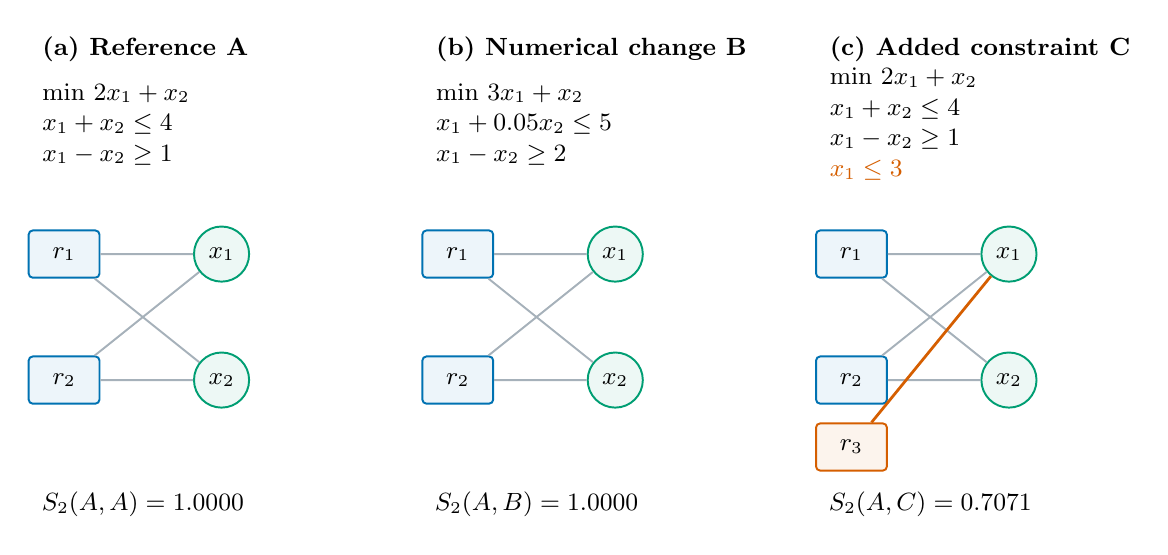
\begin{tikzpicture}[x=1cm,y=1cm]
 \begin{scope}[shift={(0,0)}]
  \node[note,anchor=west,font=\small\bfseries] at (-.15,4.2) {(a) Reference A};
  \node[note,anchor=west] at (-.15,3.25)
   {$\min\,2x_1+x_2$\\$x_1+x_2\leq4$\\$x_1-x_2\geq1$};
  \toygraph{a}{$x_1$}{$x_2$}{$r_1$}{$r_2$}{0}{}
  \node[note,anchor=north] at (1.25,-1.3) {$S_2(A,A)=1.0000$};
 \end{scope}
 \begin{scope}[shift={(5,0)}]
  \node[note,anchor=west,font=\small\bfseries] at (-.15,4.2) {(b) Numerical change B};
  \node[note,anchor=west] at (-.15,3.25)
   {$\min\,3x_1+x_2$\\$x_1+0.05x_2\leq5$\\$x_1-x_2\geq2$};
  \toygraph{b}{$x_1$}{$x_2$}{$r_1$}{$r_2$}{0}{}
  \node[note,anchor=north] at (1.25,-1.3) {$S_2(A,B)=1.0000$};
 \end{scope}
 \begin{scope}[shift={(10,0)}]
  \node[note,anchor=west,font=\small\bfseries] at (-.15,4.2) {(c) Added constraint C};
  \node[note,anchor=west] at (-.15,3.25)
   {$\min\,2x_1+x_2$\\$x_1+x_2\leq4$\\$x_1-x_2\geq1$\\
    \textcolor{graphorange}{$x_1\leq3$}};
  \toygraph{c}{$x_1$}{$x_2$}{$r_1$}{$r_2$}{1}{$r_3$}
  \node[note,anchor=north] at (1.25,-1.3) {$S_2(A,C)=0.7071$};
 \end{scope}
\end{tikzpicture}
\caption{Illustrative support graphs before the bound normalization used
for the two result tables. All variables are continuous and nonnegative (circle
nodes); all explicit rows are inequalities (rectangle nodes). Numerical
changes in B leave this graph unchanged. The additional explicit row in
C creates one node and one edge. For this teaching example only, the
common nonnegativity bounds are not drawn and $x_1\leq3$ remains an
explicit row. The score $0.7071$ therefore pertains to this illustrated
graph, not either fully normalized convention. Under bounds exclusion,
A and C instead have identical support graphs and similarity $1$.
These examples are not performance experiments.}
\label{fig:wl-encoding}
\end{figure}

\medskip
\textbf{WL refinement with the original paper's notation.}
We use the WL subtree kernel of Definition~4 in
\citet{Shervashidze2011}, with refinement as in Algorithms~1 and~2
and the input labels specified above. We compute the fixed-height
kernel through round $h$, without applying the early-stopping rule
of the isomorphism test.
Set $l_0(v)=\ell(v)$. At iteration $i\geq1$,
\[
 M_i(v)=\{\!\{l_{i-1}(u):u\in\mathcal N(v)\}\!\}.
\]
Here $\mathcal N(v)$ is the set of adjacent nodes, and double braces
denote a multiset: repeated neighbor labels are retained.
We form a signature by prefixing the sorted neighbor labels with the
node's own previous label:
\[
s_i(v)=\operatorname{concat}
\big(l_{i-1}(v),\operatorname{sort}(M_i(v))\big).
\]
Then
\[
 l_i(v)=f(s_i(v)),\qquad
 f(s_i(v))=f(s_i(w))\ \Longleftrightarrow\ s_i(v)=s_i(w).
\]
The injective dictionary implementing $f$ is shared across all 152 graphs
at each iteration, separately for each bound convention.
All nodes update synchronously from round $i-1$.
In code, a tuple stores the old label and sorted neighbor
labels; this is an unambiguous encoding of the same signature.
The compressed label identifiers are arbitrary; equal signatures receive
equal identifiers across graphs. At initialization, Algorithm~1 uses
$M_0(v):=l_0(v)=\ell(v)$; the neighbor-multiset formula applies only for
$i\geq1$. There is no $l_{-1}$ or refinement step at round zero.
Let $\Sigma_i=\{\sigma_{i1},\ldots,\sigma_{i|\Sigma_i|}\}$ be the shared
alphabet at iteration $i$, and let $c_i(G,\sigma)$ count occurrences of
label $\sigma$. The cumulative feature vector is
\[
\phi^{(h)}_{\WL}(G)=
\big(c_0(G,\sigma_{01}),\ldots,c_0(G,\sigma_{0|\Sigma_0|}),
\ldots,c_h(G,\sigma_{h1}),\ldots,c_h(G,\sigma_{h|\Sigma_h|})\big).
\]
We keep alphabets for different rounds disjoint by using
$(i,\text{label})$ as the feature key. The original subtree kernel is
\[
 k^{(h)}_{\WL}(G,G')=
 \langle\phi^{(h)}_{\WL}(G),\phi^{(h)}_{\WL}(G')\rangle
 =\sum_{i=0}^{h}\sum_{\sigma\in\Sigma_i}
 c_i(G,\sigma)c_i(G',\sigma).
\]
For reporting, we normalize this kernel:
\[
 S_h(P,Q)=
 \frac{k^{(h)}_{\WL}(G_P,G_Q)}
 {\sqrt{k^{(h)}_{\WL}(G_P,G_P)\,k^{(h)}_{\WL}(G_Q,G_Q)}}.
\]
This last normalization and the optimization-model labels are our
application choices; they are stated separately from the paper's
unnormalized kernel definition. Scores lie in $[0,1]$, with larger
values indicating closer normalized label-count vectors.

\begin{figure}[ht]
\centering
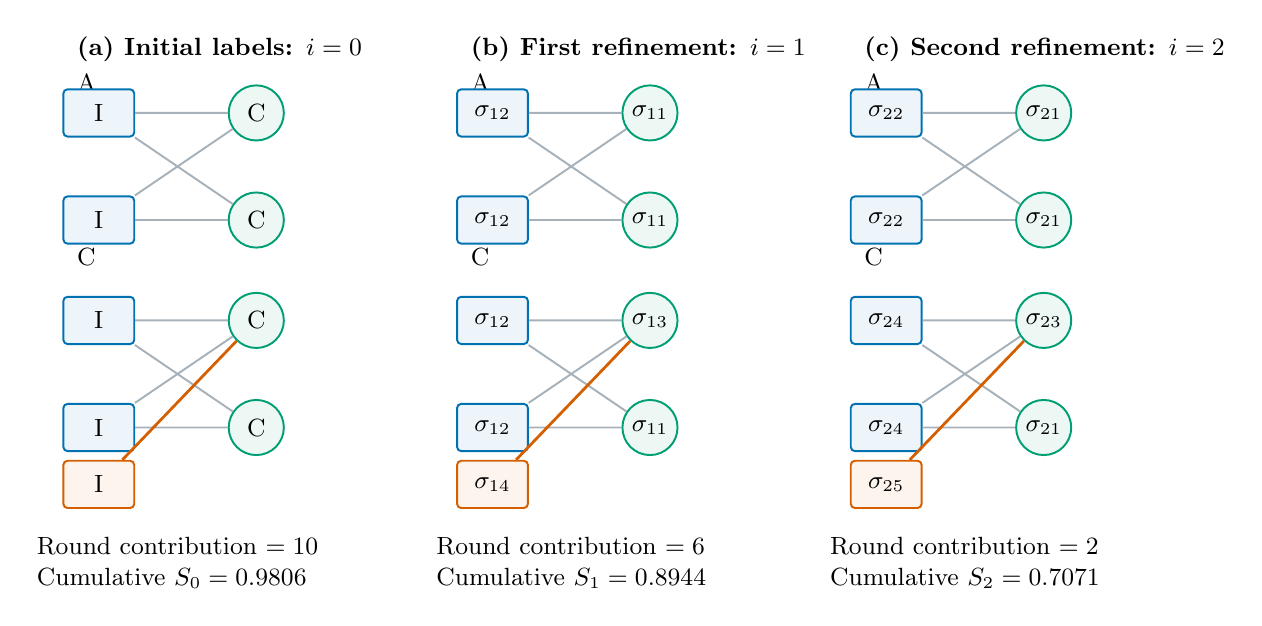
\begin{tikzpicture}[x=1cm,y=.85cm]
 \begin{scope}[shift={(0,0)}]
  \node[note,anchor=west,font=\small\bfseries] at (-.15,2.55) {(a) Initial labels: $i=0$};
  \node[note,anchor=west] at (-.15,2.05) {A};
  \toygraph{d}{C}{C}{I}{I}{0}{}
  \node[note,anchor=west] at (-.15,-.55) {C};
  \begin{scope}[shift={(0,-3.1)}]
   \toygraph{e}{C}{C}{I}{I}{1}{I}
  \end{scope}
  \node[note,anchor=north] at (1.25,-4.6)
   {Round contribution $=10$\\Cumulative $S_0=0.9806$};
 \end{scope}
 \begin{scope}[shift={(5,0)}]
  \node[note,anchor=west,font=\small\bfseries] at (-.15,2.55) {(b) First refinement: $i=1$};
  \node[note,anchor=west] at (-.15,2.05) {A};
  \toygraph{f}{$\sigma_{11}$}{$\sigma_{11}$}{$\sigma_{12}$}{$\sigma_{12}$}{0}{}
  \node[note,anchor=west] at (-.15,-.55) {C};
  \begin{scope}[shift={(0,-3.1)}]
   \toygraph{g}{$\sigma_{13}$}{$\sigma_{11}$}{$\sigma_{12}$}{$\sigma_{12}$}{1}{$\sigma_{14}$}
  \end{scope}
  \node[note,anchor=north] at (1.25,-4.6)
   {Round contribution $=6$\\Cumulative $S_1=0.8944$};
 \end{scope}
 \begin{scope}[shift={(10,0)}]
  \node[note,anchor=west,font=\small\bfseries] at (-.15,2.55) {(c) Second refinement: $i=2$};
  \node[note,anchor=west] at (-.15,2.05) {A};
  \toygraph{h}{$\sigma_{21}$}{$\sigma_{21}$}{$\sigma_{22}$}{$\sigma_{22}$}{0}{}
  \node[note,anchor=west] at (-.15,-.55) {C};
  \begin{scope}[shift={(0,-3.1)}]
   \toygraph{j}{$\sigma_{23}$}{$\sigma_{21}$}{$\sigma_{24}$}{$\sigma_{24}$}{1}{$\sigma_{25}$}
  \end{scope}
  \node[note,anchor=north] at (1.25,-4.6)
   {Round contribution $=2$\\Cumulative $S_2=0.7071$};
 \end{scope}
\end{tikzpicture}
\caption{WL propagation in the added-constraint example. C and I abbreviate
\texttt{V:C} and \texttt{R:I}; $\sigma_{ij}$ is the $j$th compressed label
at round $i$. Matching symbols within a round have matching signatures.
The new row first changes $x_1$'s label, then changes the labels of its
neighboring original rows. Round contributions are
$\sum_{\sigma\in\Sigma_i}c_i(G_A,\sigma)c_i(G_C,\sigma)$.
Scores use cumulative counts from rounds $0,\ldots,h$. As in
Figure~\ref{fig:wl-encoding}, this illustration leaves the added singleton
row explicit and does not normalize the common nonnegativity bounds.}
\label{fig:wl-rounds}
\end{figure}


\medskip
\textbf{Worked example: the A--C calculation.}
Write $\nu=\texttt{V:C}$ and $\rho=\texttt{R:I}$.
Superscripts identify the graph. In A, each variable is adjacent to
$r_1^A,r_2^A$, and each row is adjacent to $x_1^A,x_2^A$.
In C, $x_1^C$ is adjacent to all three rows, $x_2^C$ to the first two,
and $r_3^C$ only to $x_1^C$.

At round zero, variable labels are $\nu$ and row labels are $\rho$.
The count vectors in order $(\nu,\rho)$ are $(2,2)$ for A and
$(2,3)$ for C. The cross contribution is $10$, and their self
contributions are $8$ and $13$.

At round one, the following four groups cover every node.
The bracketed expression is the signature $s_1(v)$, formed from
the node's old label and its sorted neighbor multiset:
\[
\begin{aligned}
v\in\{x_1^A,x_2^A,x_2^C\}:&
\quad M_1(v)=\{\!\{\rho,\rho\}\!\},&
l_1(v)&=f(\langle\nu;\rho,\rho\rangle)=\sigma_{11},\\
v\in\{r_1^A,r_2^A,r_1^C,r_2^C\}:&
\quad M_1(v)=\{\!\{\nu,\nu\}\!\},&
l_1(v)&=f(\langle\rho;\nu,\nu\rangle)=\sigma_{12},\\
v=x_1^C:&
\quad M_1(v)=\{\!\{\rho,\rho,\rho\}\!\},&
l_1(v)&=f(\langle\nu;\rho,\rho,\rho\rangle)=\sigma_{13},\\
v=r_3^C:&
\quad M_1(v)=\{\!\{\nu\}\!\},&
l_1(v)&=f(\langle\rho;\nu\rangle)=\sigma_{14}.
\end{aligned}
\]
Thus the count vectors in alphabet order
$(\sigma_{11},\sigma_{12},\sigma_{13},\sigma_{14})$ are
$(2,2,0,0)$ and $(1,2,1,1)$.
The cross contribution is $2\cdot1+2\cdot2=6$;
self contributions are $8$ and $7$.

At round two, the five groups below again cover every node:
\[
\begin{aligned}
v\in\{x_1^A,x_2^A,x_2^C\}:&
\quad M_2(v)=\{\!\{\sigma_{12},\sigma_{12}\}\!\},\\[-2pt]
&\quad l_2(v)=f(\langle\sigma_{11};\sigma_{12},\sigma_{12}\rangle)
=\sigma_{21},\\
v\in\{r_1^A,r_2^A\}:&
\quad M_2(v)=\{\!\{\sigma_{11},\sigma_{11}\}\!\},\\[-2pt]
&\quad l_2(v)=f(\langle\sigma_{12};\sigma_{11},\sigma_{11}\rangle)
=\sigma_{22},\\
v=x_1^C:&
\quad M_2(v)=\{\!\{\sigma_{12},\sigma_{12},\sigma_{14}\}\!\},\\[-2pt]
&\quad l_2(v)=f(\langle\sigma_{13};
\sigma_{12},\sigma_{12},\sigma_{14}\rangle)=\sigma_{23},\\
v\in\{r_1^C,r_2^C\}:&
\quad M_2(v)=\{\!\{\sigma_{13},\sigma_{11}\}\!\},\\[-2pt]
&\quad l_2(v)=f(\langle\sigma_{12};\sigma_{11},\sigma_{13}\rangle)
=\sigma_{24},\\
v=r_3^C:&
\quad M_2(v)=\{\!\{\sigma_{13}\}\!\},\\[-2pt]
&\quad l_2(v)=f(\langle\sigma_{14};\sigma_{13}\rangle)=\sigma_{25}.
\end{aligned}
\]
The original rows in C see different round-one variable labels
$\sigma_{13},\sigma_{11}$; A's original rows see
$\sigma_{11},\sigma_{11}$. Hence their round-two labels differ.
However, $x_2^C$ still reads its neighbors' \emph{round-one}
labels, both $\sigma_{12}$, rather than their newly computed
round-two labels. It therefore matches A's variables.
Refinement adds no nodes or edges.

In alphabet order $(\sigma_{21},\ldots,\sigma_{25})$, the round-two
counts are $(2,2,0,0,0)$ and $(1,0,1,2,1)$.
Their cross contribution is $2$, and self contributions are $8,7$.
The cumulative feature vectors and similarities are
\[
\begin{aligned}
\phi^{(2)}_{\WL}(G_A)&=(2,2\,;\;2,2,0,0\,;\;2,2,0,0,0),\\
\phi^{(2)}_{\WL}(G_C)&=(2,3\,;\;1,2,1,1\,;\;1,0,1,2,1),\\
S_0(A,C)&=\frac{10}{\sqrt{8\cdot13}}=0.9806,\\
S_1(A,C)&=\frac{10+6}{\sqrt{(8+8)(13+7)}}=0.8944,\\
S_2(A,C)&=\frac{10+6+2}{\sqrt{(8+8+8)(13+7+7)}}=0.7071.
\end{aligned}
\]
Semicolons separate the rounds. The calculation uses all rounds up to
$h$, rather than just the last round, and was checked against the
benchmark WL module. Moving $x_1\leq3$ into excluded \texttt{Bounds}
makes A's and C's graphs identical, giving similarity $1$ despite
different feasible sets. Excluding bounds therefore does not
universally decrease similarity.

A score of $1$ means proportional feature vectors, not model equivalence.
For example, one eight-node alternating cycle and two disjoint
four-node alternating cycles have identical typed WL counts at every
depth despite different connectivity.

\medskip
\textbf{Reference matching and reproducibility.}
For a test formulation $P$ of category $g(P)$, let
$\mathcal R_{g(P)}$ denote its category's reference pool and
$\mathcal R$ the full collection. Within each bound convention,
\[
 S_{\rm same}(P)=\max_{R\in\mathcal R_{g(P)}}S_2(P,R),
 \qquad
 S_{\rm all}(P)=\max_{R\in\mathcal R}S_2(P,R).
\]
Nearest-reference matching means maximum similarity.
Each category's median and mean summarize these per-instance maxima;
the all-instance row pools individual scores, rather than averaging
category medians or means.
There is one reference each for NRM, RA, TP, AP, and UFLP, eight for
Mixture, and two for Others. Mixture matching does not merge Others.
Different candidate-pool sizes affect the maxima, and Others is a
heterogeneous pool rather than one modeling archetype.
All-reference scores concern the available collection, not necessarily
references retrieved during individual pipeline runs.
The 36 variants contain 3 AP, 3 UFLP, 17 Mixture, and 13 Others
instances; there are no NRM, RA, or TP variants in this set.

Both normalization procedures cover all 152 formulations.
Source LP and input CSV hashes remained unchanged.
Checks covered effective variable domains and bounds, retained rows,
objective sense and constants, and multiobjective metadata.
Each normalized model was exported to LP and MPS and read back.
Prior reconstruction of all 15 reference CSV Code fields verified
Code-to-LP correspondence; this does not independently certify every
natural-language modeling decision.
For explicit-bound conversion, 151 original/converted pairs returned
matching optimal objectives. The remaining pair, Other6, produced
feasible solutions with matching objectives within tolerance but did
not prove optimality within the time limit.
These checks concern conversion, not LLM accuracy.

We keep the existing primary depth $h=2$, report both bound conventions,
and do not choose settings to minimize similarity.
Symmetry, unit self-similarity, node-reordering invariance, and
disjoint-replication invariance were checked.
No learned classifier or fitted similarity threshold is used.

\begin{table}[H]
\centering\small\color{replyblue}
\caption{WL similarities with effective variable bounds stored in \texttt{Bounds} and excluded from the graph.}
\label{tab:ae-wl-bounds-excluded}
\setlength{\tabcolsep}{6pt}
\begin{tabular}{@{}lrrrr@{}}
\toprule
Category & Tests & Median $S_{\rm same}$ & Mean $S_{\rm same}$ &
Median $S_{\rm all}$\\
\midrule
\multicolumn{5}{@{}l}{\textbf{(a) Original Large-Scale-OR instances}}\\
NRM & 25 & 0.3234 & 0.3234 & 0.3330\\
RA & 22 & 0.6562 & 0.6564 & 0.6562\\
TP & 9 & 0.6240 & 0.6314 & 0.6343\\
AP & 5 & 0.0508 & 0.0551 & 0.4424\\
UFLP & 14 & 0.5503 & 0.5557 & 0.5503\\
Mixture & 18 & 0.3983 & 0.4499 & 0.5025\\
Others & 8 & 0.2584 & 0.3025 & 0.3811\\
\midrule
\textbf{All instances} & \textbf{101} & \textbf{0.5065} & \textbf{0.4632} & \textbf{0.5340}\\
\midrule
\multicolumn{5}{@{}l}{\textbf{(b) Task variants}}\\
NRM & 0 & --- & --- & ---\\
RA & 0 & --- & --- & ---\\
TP & 0 & --- & --- & ---\\
AP & 3 & 0.3569 & 0.3582 & 0.3569\\
UFLP & 3 & 0.1981 & 0.1972 & 0.3078\\
Mixture & 17 & 0.6665 & 0.6157 & 0.6665\\
Others & 13 & 0.2373 & 0.2993 & 0.4359\\
\midrule
\textbf{All instances} & \textbf{36} & \textbf{0.4325} & \textbf{0.4451} & \textbf{0.5588}\\
\bottomrule
\end{tabular}
\par\vspace{4pt}
\parbox{\linewidth}{\footnotesize
All values use cumulative rounds $0$--$2$ and cosine normalization;
higher means closer under this graph convention.
Each score first maximizes similarity over the specified reference pool.
All-instance rows pool the individual scores.
Dashes denote absent categories, not zero similarity.
Scores are not percentages of shared constraints or accuracy measures.}
\end{table}

\begin{table}[H]
\centering\small\color{replyblue}
\caption{WL similarities with effective finite variable bounds also represented as explicit constraint nodes.}
\label{tab:ae-wl-bounds-included}
\setlength{\tabcolsep}{6pt}
\begin{tabular}{@{}lrrrr@{}}
\toprule
Category & Tests & Median $S_{\rm same}$ & Mean $S_{\rm same}$ &
Median $S_{\rm all}$\\
\midrule
\multicolumn{5}{@{}l}{\textbf{(a) Original Large-Scale-OR instances}}\\
NRM & 25 & 0.6097 & 0.6097 & 0.8494\\
RA & 22 & 0.8335 & 0.8210 & 0.8335\\
TP & 9 & 0.8245 & 0.8275 & 0.8293\\
AP & 5 & 0.2169 & 0.2166 & 0.6146\\
UFLP & 14 & 0.7740 & 0.7735 & 0.7740\\
Mixture & 18 & 0.6779 & 0.6993 & 0.7723\\
Others & 8 & 0.6477 & 0.6060 & 0.6790\\
\midrule
\textbf{All instances} & \textbf{101} & \textbf{0.7271} & \textbf{0.6940} & \textbf{0.8335}\\
\midrule
\multicolumn{5}{@{}l}{\textbf{(b) Task variants}}\\
NRM & 0 & --- & --- & ---\\
RA & 0 & --- & --- & ---\\
TP & 0 & --- & --- & ---\\
AP & 3 & 0.6079 & 0.6074 & 0.6109\\
UFLP & 3 & 0.5615 & 0.5608 & 0.6346\\
Mixture & 17 & 0.8340 & 0.8141 & 0.8340\\
Others & 13 & 0.6174 & 0.6107 & 0.7157\\
\midrule
\textbf{All instances} & \textbf{36} & \textbf{0.6793} & \textbf{0.7023} & \textbf{0.7676}\\
\bottomrule
\end{tabular}
\par\vspace{4pt}
\parbox{\linewidth}{\footnotesize
All values use cumulative rounds $0$--$2$ and cosine normalization;
higher means closer under this graph convention.
Each score first maximizes similarity over the specified reference pool.
All-instance rows pool the individual scores.
Dashes denote absent categories, not zero similarity.
Scores are not percentages of shared constraints or accuracy measures.}
\end{table}


\medskip
\textbf{Results and interpretation.}
With bounds retained only in \texttt{Bounds}
(Table~\ref{tab:ae-wl-bounds-excluded}), the 101-instance same-category
median is $0.5065$, its mean is $0.4632$, and the all-reference median
is $0.5340$. With bounds also represented as constraint rows
(Table~\ref{tab:ae-wl-bounds-included}), the corresponding values are
$0.7271$, $0.6940$, and $0.8335$.
Resemblance therefore varies by category and by the information
included in the graph.

RA's same-category median changes from $0.6562$ to $0.8335$,
TP's from $0.6240$ to $0.8245$, and UFLP's from $0.5503$ to
$0.7740$ when bounds are included.
Common bound rows add similarly labeled leaf nodes and alter the
refinement signatures of neighboring variables.
They increase category medians on these data, although the A--C
example demonstrates that this direction is not universal.
Changing the storage location of a bound does not change the
mathematical problem: the diagnostics measure different selected
representations.

Allowing any reference also reveals resemblance missed by
same-category matching. AP's median rises from $0.0508$ to $0.4424$
under bounds exclusion, and from $0.2169$ to $0.6146$ under bounds
inclusion. Mixture's corresponding values rise from $0.3983$ to
$0.5025$, and from $0.6779$ to $0.7723$.
A difference from the designated category template is therefore
not a difference from every available reference.

The variant same-category median is $0.4325$ under bounds exclusion
and $0.6793$ under inclusion; all-reference medians are $0.5588$
and $0.7676$. Under exclusion, category medians range from $0.1981$
for UFLP to $0.6665$ for Mixture.
Because the original and variant sets have different category
compositions, their pooled medians do not establish that every
variant is less similar, more complex, or farther from its own original.

Three qualifications are especially relevant to the AE's concern.
\begin{enumerate}
\item \textbf{NRM reflects a reference revision.}
All singleton restrictions in the 25 NRM tests become bounds.
Under exclusion, their graphs retain integer variable nodes but
have no row nodes or edges.
The current NRM reference contains a synthetic shared-dispatch row
coupling four variables, added in an earlier revision after
inspecting reference resemblance. This largely explains the score
$0.3234$. Removing only this row from a separate diagnostic copy
restores all 25 scores to $1$ under either normalized convention.
The lower NRM scores describe the revised reference; they do not
independently establish test heterogeneity or robustness to new
test-side requirements.

\item \textbf{AP includes a variable-domain difference.}
The five original AP exports use continuous variables, whereas their
reference uses binary variables. This changes the initial labels
and subsequent refinements. The low score does not by itself
establish different business requirements.
Under standard assignment assumptions, a continuous relaxation can
have integral optimal solutions; its graph encoding still differs here.

\item \textbf{WL is not a calibrated novelty test.}
No universal high/low threshold is assumed.
A score of $0.5065$ is not $50.65\%$ shared constraints or business rules.
One original UFLP instance attains similarity $1$ under both
conventions, so overlap remains present.
The $h=1,2,3$ pooled same-category medians are
$0.6748,0.5065,0.4005$ with bounds excluded and
$0.9007,0.7271,0.5782$ with bounds included.
We retain $h=2$ without selecting depth to lower the score.
\end{enumerate}

The diagnostics quantify local structural differences and shared
patterns, partially addressing the possibility that category labels
or semantic comparisons conceal formulation overlap.
They do not rule out shared templates or prove generalization to
unseen archetypes. Objectives, coefficient values and signs, and
right-hand-side changes are outside this encoding.

\medskip
\textbf{Complementary performance evidence for robustness.}
To address performance, we also evaluated task variants, LOTO
reference withholding, and forced routing.
These interventions change the task or its available modeling
support; WL itself only measures formulation resemblance.

The saved 36-variant evaluation completed 30 of 36 instances and
matched the reference objective on 29 of 36 ($80.56\%$).
In the saved GPT-4.1 LOTO examples-and-route experiment,
matching category examples were removed and the corresponding
execution route disabled. The pipeline completed 94 of 101
instances and matched the objective on 88 of 101 ($87.13\%$),
compared with 95 of 101 ($94.06\%$) for that experiment's saved
full baseline, a decrease of $6.93$ percentage points.
This evaluates a specified withholding intervention, not complete
removal of all prior knowledge about the category.

The saved forced-routing evaluation applies six execution routes
to each of the 101 problems.
Among the 505 assignments to a route different from the designated
route, 474 returned a solution and 431 matched the reference
objective ($85.35\%$ of all 505 assignments).
These are repeated assignments to 101 problems, not 505 independent
benchmark problems. Forced routing fixes an execution route;
route withholding instead lets the classifier choose among the
remaining routes. The interventions are distinct.

All objective-match rates use relative and absolute tolerances
$10^{-4}$, with failures included in the denominator.
Objective matching is a performance indicator, not proof that every
constraint and modeling decision is correct.
The variant, LOTO, and forced-routing records come from their
respective saved implementation snapshots; their rates should not
be pooled or treated as a common-version head-to-head comparison.
The bound-normalization analysis did not rerun LLM evaluations.

Together, these structural diagnostics and performance experiments
provide complementary evidence of resilience within the evaluated
settings, while exposing remaining failures.
We therefore qualify the robustness claim: the evidence supports
performance beyond reliance on a single intact same-category
reference template, but does not establish universal robustness
to arbitrary new constraints, objectives, or business requirements.
\endgroup

\begin{thebibliography}{5}
\bibitem[Shervashidze et~al.(2011)]{Shervashidze2011}
Shervashidze, N., Schweitzer, P., van Leeuwen, E.~J., Mehlhorn, K.,
and Borgwardt, K.~M. (2011).
Weisfeiler--Lehman graph kernels.
\emph{Journal of Machine Learning Research}, 12(77), 2539--2561.
\url{https://jmlr.org/papers/v12/shervashidze11a.html}.

\bibitem[Gasse et~al.(2019)]{Gasse2019}
Gasse, M., Ch\'{e}telat, D., Ferroni, N., Charlin, L., and Lodi, A. (2019).
Exact combinatorial optimization with graph convolutional neural networks.
\emph{Advances in Neural Information Processing Systems}, 32.
\url{https://arxiv.org/abs/1906.01629}.

\bibitem[Hosny and Reda(2024)]{Hosny2024}
Hosny, A., and Reda, S. (2024).
Automatic MILP solver configuration by learning problem similarities.
\emph{Annals of Operations Research}, 339, 909--936.
\url{https://doi.org/10.1007/s10479-023-05508-x}.

\bibitem[Chen et~al.(2023)]{Chen2023}
Chen, Z., Liu, J., Wang, X., Lu, J., and Yin, W. (2023).
On representing mixed-integer linear programs by graph neural networks.
\emph{International Conference on Learning Representations}.
\url{https://arxiv.org/abs/2210.10759}.

\bibitem[Jahin et~al.(2026)]{Jahin2026}
Jahin, M.~A., Knoblock, C.~A., and Pujara, J. (2026).
A Weisfeiler--Leman characterization of global-attention graph transformers
for mixed-integer linear programs.
arXiv:2607.17570. The arXiv record reports acceptance at TAG-DS 2026.
\url{https://arxiv.org/abs/2607.17570}.
\end{thebibliography}
\end{document}
